\section{Der Algorithmus}

Wie in der Einleitung schon erw"ahnt worden ist, arbeitet der Simplex-Downhill Algorithmus ohne Ableitungen.
Warum das funktioniert wird klar, wenn man sich vorstellt, dass das Simplex selber auf der Zielfunktion liegt und sozusagen die Ableitung approximiert. Sucht der Algorithmus ein Minimum, so bewegt er sich nat"urlich abw"arts (downhill), was auch seine Namensgebung erkl"art.
Der Algorithmus ist natürlich ebenfalls in der Lage nach Maxima zu suchen indem die Zielfunktion einfach invertiert wird.
Im Folgenden wir immer davon ausgegangen, dass ein Minimum gesucht wird.

\subsection{Hauptablauf}
Der Algorithmus besteht aus einer Initialisierung, einer Iterationsschlaufe und einer Abbruchbedingung (siehe \figref{fig:downhillalgo1})

\begin{figure}[h]
\resizebox{1\textwidth}{!}{
\providecommand{\highlight}{white}
\begin{tikzpicture}[node distance = 1.7cm,every node/.style={rectangle,fill=white},
  block/.style={draw,align=center},
  highlight/.style={draw,fill=\highlight},
  line/.style = {draw,-latex'}
]

\node (start) [block] {N+1 Startpunkte $x_i$ w"ahlen (Simplex bilden)};

\node (a1) [block, below of=start] { $y_i = f(x_i)$ berechnen};

\node (a2) [block, below of=a1] { Bestes ($y_{min}$) und schlechtestes ($y_{max}$) $y_i$ bestimmen};

\node (a3) [block, below of=a2,text width=5cm]{Abbruchbedingung erf"ullt?};

\node (ende) [block, below of=a3] {Ende};

\node (a4) [highlight, left of=a3, node distance=6cm] {Neuer Simplex bilden};



\path[line] (start) -- (a1);
\path[line] (a1) -> (a2);
\path[line] (a2) -> (a3);

\path[line] (a3) -> node{ja} (ende);
\path[line] (a3) -> node{nein} (a4);

\path[line] (a4)  |-  (a1.west);

\end{tikzpicture}
}

\caption{"Ubersicht des Algorithmus}
\label{fig:downhillalgo1}
\end{figure}

Zu Beginn wird ein Simplex mit den Ecken $x_i$ gebildet.
Zu den gew"ahlten $x_i$ werden nun die dazu geh"origen $y_i$ der Zielfunktion ausgerechnet.

Aus den erhaltenen Funktionswerten wird der beste $y_{min}$, der schlechteste $y_{max}$ sowie der Mittelwert ohne $x_{max}$ extrahiert.

Diese werden f"ur die Abbruchbedingung \chapref{sec:downhillAbbruch} und zur Bildung des neuen Simplex ben"otigt, siehe \chapref{sec:downhillModi}.

Hat man das Simplex auf der Zielfunktion platziert, werden die berechneten Testpunkte gepr"uft, wobei der schlechteste dieser Punkte mittels gewisser ''Taktiken`` ersetzt wird. Dies wird solange fort gef"uhrt, bis das gew"unschte Ergebnis erreicht worden ist, also eine Abbruchbedingung erfüllt ist.

\subsection{Abbruchbedingungen}
\label{sec:downhillAbbruch}
Es k"onnen diverse Abbruchbedingungen f"ur den Downhill-Simplex verwendet werden
\begin{itemize}
\item Der Wert von $y_{min}$: Es kann abgebrochen werden, sobald ein gewisser Wert unterschritten wird
\item Werte von $x_i$: Sobald alle $x_i$ nahe beieinander sind, wird abgebrochen, da es keine grosse "Anderung mehr gibt.
\item Maximale Iterationszahl: Als Notfall wenn nicht konvergiert wird
\end{itemize}

Es empfiehlt sich eine Kombination der Abbruchbedingungen, um die Iterationszahl m"oglichst gering zu halten.
Im Allgemeinen ist es Empfehlenswert die $x_i$ und Anzahl Iterationen zu verwenden, da so kein Wissen "uber die Art des Minimums der Zielfunktion ben"otigt wird.

Ist die gew"ahlte Abbruchbedingung erf"ullt, ist der Algorithmus am Ende.
Es ist nat"urlich eher Zufall, wenn man gleich bei der ersten Wahl des Simplex das Minima trifft, meistens hat man es nicht getroffen und es wird nun auf Grund des gew"ahlten Simplex gem"ass \chapref{sec:downhillModi} ein neues Simplex gebildet.

\subsection{Neuen Simplex bilden}
\label{sec:downhillModi}

Das Auswahlverfahren des neuen Simplex unterliegt eine Reihe von Entscheidungen aufgrund der gegebenen Eckpunkte sowie deren Funktionswerte.
In \figref{fig:downhillalg2} ist dieser Entscheidungsbaum ersichtlich.

\begin{figure}[h]
\usetikzlibrary{shapes}
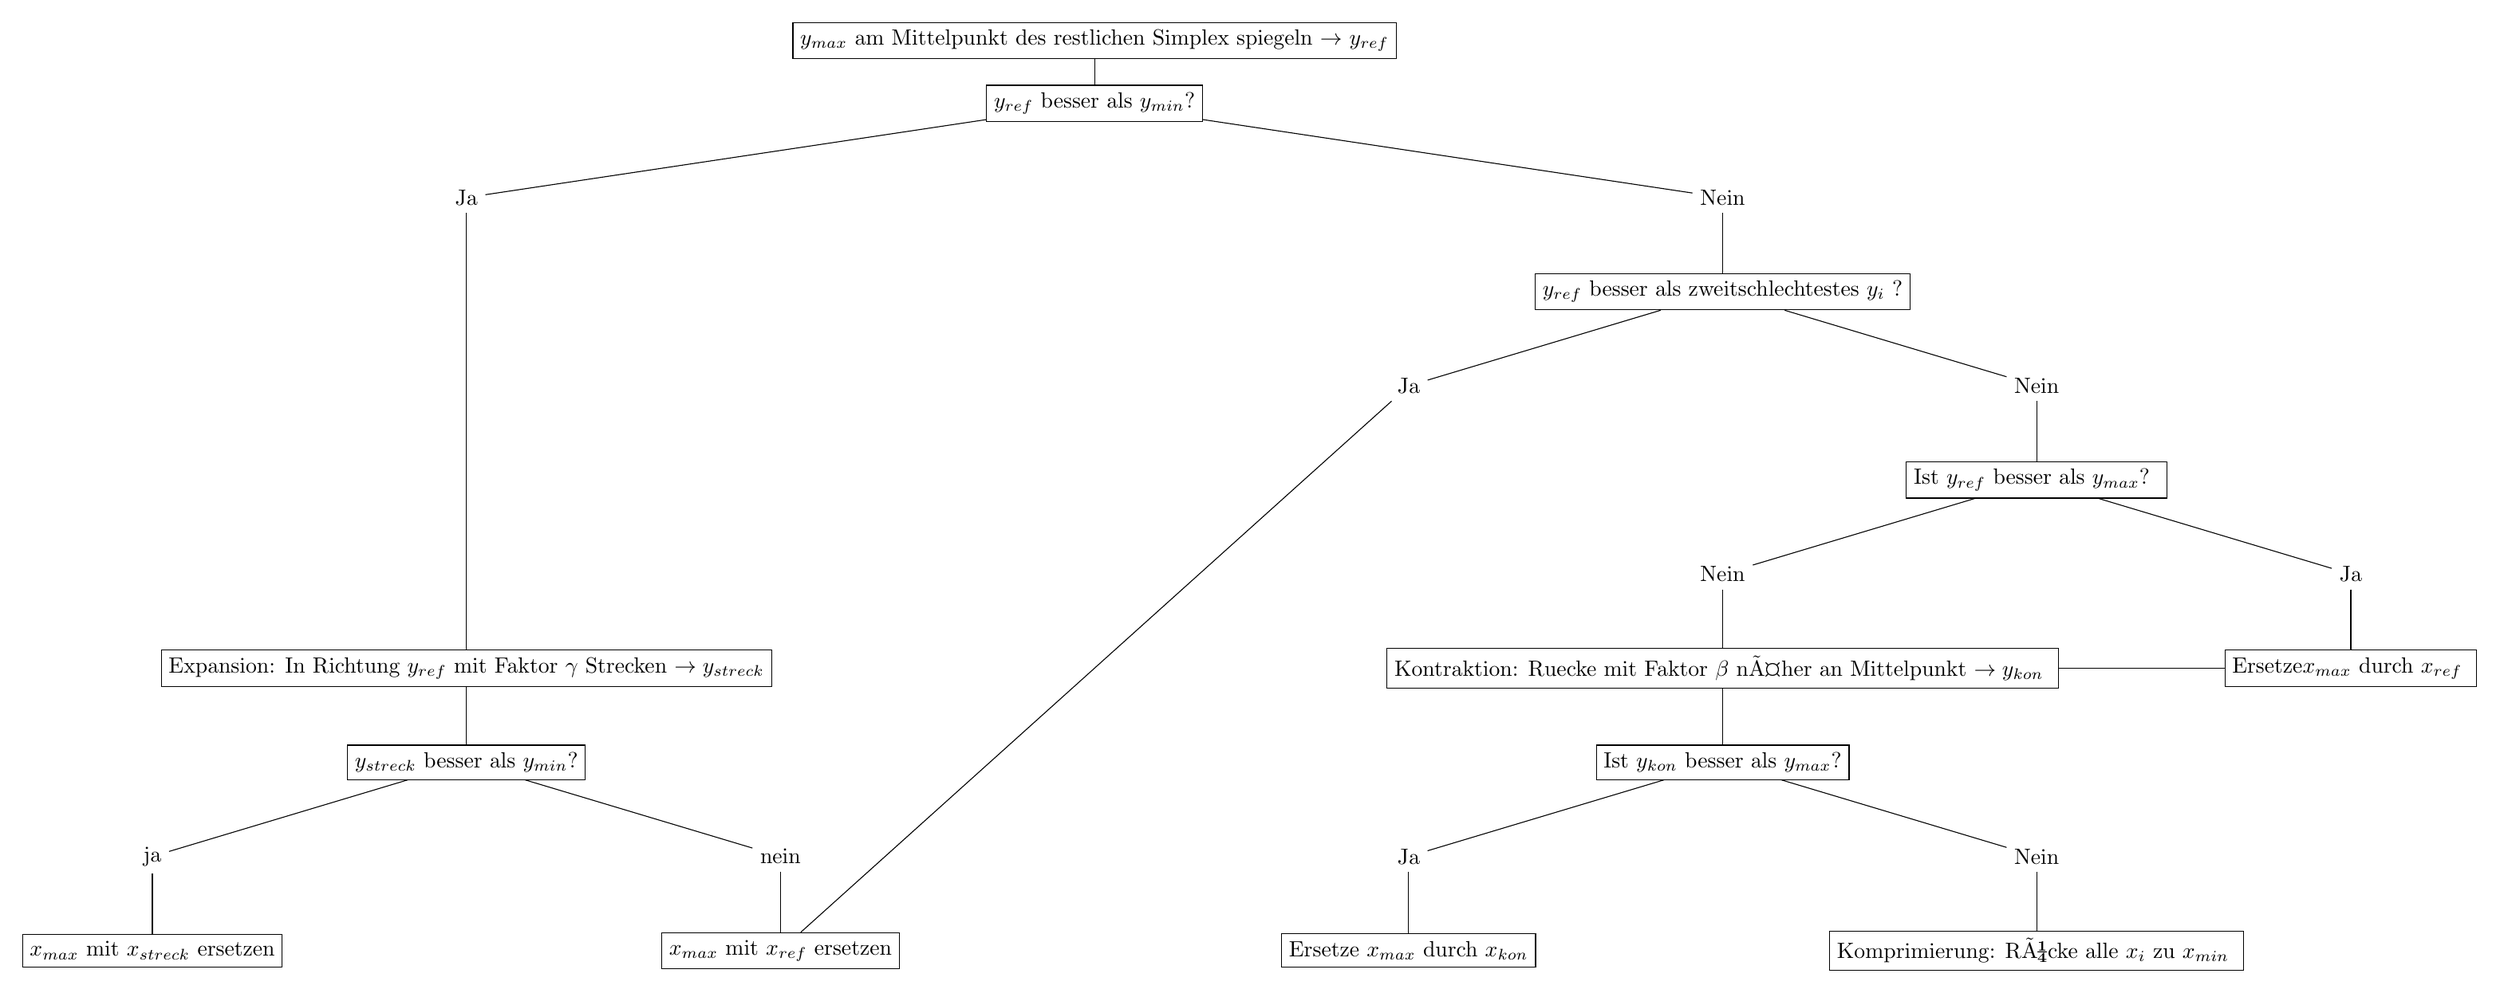
\begin{tikzpicture}[
  top/.style={draw,align=center},
  med/.style={draw,align=center},
  fin/.style={ellipse,draw,align=center}
]

\tikzstyle{level 1}=[sibling distance=200mm,align=center]
\tikzstyle{level 2}=[sibling distance=100mm,align=center]
%\tikzstyle{level 3}=[sibling distance=100mm]


\node (start) at (0,1)[draw] {$y_{max}$ am Mittelpunkt des restlichen Simplex spiegeln $\rightarrow$ $y_{ref}$};

\node[top](top){$y_{ref}$ besser als  $y_{min}$?}
	child { node {Ja} child {child { child  { child { child {
		node[med] {Expansion: In Richtung $y_{ref}$ mit Faktor $\gamma$ Strecken  $\rightarrow y_{streck} $}
		child{
			node[med]  {$y_{streck}$ besser als $y_{min}$?}
			child { node {ja}
			child { node [med]{$x_{max}$ mit $x_{streck}$ ersetzen} }}
			child { node {nein}
			child { node(a2) [med]{$x_{max}$ mit $x_{ref}$ ersetzen} }}
		}
	}}}}}}
	child {
		node {Nein}
		child  {
		node [med] {$y_{ref}$ besser als zweitschlechtestes $y_i$ ?}
		child { node (b1) [] {Ja} }
		child { node {Nein} 
		child { node[med] {Ist $y_{ref}$ besser als $y_{max}$? }
			child {node{Nein}
				child { node (kont)[med] {Kontraktion: Ruecke mit Faktor $\beta$ näher an Mittelpunkt $\rightarrow y_{kon}$ }
					child { node[med]  {Ist $y_{kon}$ besser als $y_{max}$?}
						child {node {Ja}
							child {node[med] {Ersetze $x_{max}$ durch $x_{kon}$}}
						}
						child {node {Nein}
							child {node[med] {Komprimierung:  Rücke alle $x_i$ zu $x_{min}$ } }
						}
					}
				}
			}
			child {node {Ja}
				child { node (zukont)[med] {Ersetze$ x_{max}$ durch $x_{ref}$ } }
			}
		}
		}
	}
	}
;
\draw (zukont) -- (kont);
\draw (b1) -- (a2);
\draw (start) --(top);

\end{tikzpicture}

\caption{Algorithmus zur Auswahl der Modifikation}
\label{fig:downhillalg2}
\end{figure}

Die M"oglichkeiten das Simplex soweit zu ver"andern, dass es den optimalen Punkt findet, sind begrenzt.
Die Darstellungen beziehen sich hierbei auf einen Simplex der zweiten Dimension (Dreieck), nat"urlich gelten diese Modifikationen auch f"ur einen n-dimensionalen Simplex.

\begin{figure}[h]
	\centering
	\input{../bilder/start.tex}%
  	\caption{Simplex im zweidimensionalen Raum}%
	\label{fig:downhillStart}
\end{figure}

Der Algorithmus w"ahlt auf Grund der Werte der Startsimplex (siehe \figref{fig:downhillStart}) beziehungsweise deren Zielfunktionswerte die Modifikationsart aus.

\subsubsection{Reflexion}

Zu Beginn wird das Simplex ziemlich grob behandelt, indem man erst einmal durch Reflexion versucht, weg vom schlechtesten Punkt zu kommen.

Bei der Reflexion wird der schlechteste Punkt $x_{max}$ am Schwerpunkt $x_m$ des restlichen Simplex gespiegelt und mit einem Faktor $\alpha$ gewichtet:

\begin{equation}
x_m = \left(\sum_1^{N+1} x_i - x_{max}\right) \frac{1}{N} \quad N = \text{Anzahl Dimensionen}
\end{equation}

\begin{equation}
x_{ref} = x_m + \alpha \cdot (x_m-x_{max})
\end{equation}

Man kann sich dieses Vorgehen als Approximation der Steigung mittels einer Ebene vorstellen.
Es wird in Richtung der Steigung dieser Ebene abgestiegen um einen besseren Punkt zu finden.

Die Reflexion wird immer durchgef"uhrt, da die folgenden Modifikationen den Punkt $x_{ref}$ ben"otigen.

\begin{figure}[h]
	\centering
	\input{../bilder/reflexion.tex}%
  	\caption{Reflexion}%
	\label{fig:Reflexion}%
\end{figure}

\subsubsection{Expansion}
War die Reflektion erfolgreich und der neue Wert $y_{ref}$ ist besser als $y_{min}$ wird in diese Richtung weiter gestreckt, um das Simplex in die scheinbar richtige Richtung zu treiben.
Dazu wird bei der Expansion der Schwerpunkt $x_m$ mit dem Faktor $\gamma$ in Richtung $x_{ref}$ gestreckt.

\begin{equation}
x_{streck} = x_{ref} + \gamma \cdot (x_{ref}-x_{m})
\end{equation}
\begin{figure}[h]
	\centering
	\resizebox{1\textwidth}{!}{
\definecolor{uuuuuu}{rgb}{0.27,0.27,0.27}
\definecolor{zzttqq}{rgb}{0.6,0.2,0}
\definecolor{qqqqff}{rgb}{0,0,1}
\begin{tikzpicture}[line cap=round,line join=round,>=triangle 45,x=1.0cm,y=1.0cm]
\clip(4.51,0.05) rectangle (11.48,4.25);
\fill[color=zzttqq,fill=zzttqq,fill opacity=0.1] (5.74,3) -- (10.36,4) -- (11,2) -- cycle;
\fill[color=zzttqq,fill=zzttqq,fill opacity=0.1] (5.74,3) -- (6.38,1) -- (11,2) -- cycle;
\fill[color=zzttqq,fill=zzttqq,fill opacity=0.1] (5.74,3) -- (5.39,0.25) -- (11,2) -- cycle;
\draw [color=zzttqq] (5.74,3)-- (10.36,4);
\draw [color=zzttqq] (10.36,4)-- (11,2);
\draw [color=zzttqq] (11,2)-- (5.74,3);
\draw (8.37,2.5)-- (6.38,1);
\draw (8.37,2.5)-- (5.39,0.25);
\draw [color=zzttqq] (5.74,3)-- (6.38,1);
\draw [color=zzttqq] (6.38,1)-- (11,2);
\draw [color=zzttqq] (11,2)-- (5.74,3);
\draw [color=zzttqq] (5.74,3)-- (5.39,0.25);
\draw [color=zzttqq] (5.39,0.25)-- (11,2);
\draw [color=zzttqq] (11,2)-- (5.74,3);
\begin{scriptsize}
\fill [color=qqqqff] (5.74,3) circle (1.5pt);
\draw[color=qqqqff] (5.75,3.11) node {$x_{min}$};
\fill [color=qqqqff] (10.36,4) circle (1.5pt);
\draw[color=qqqqff] (10.53,4.07) node {$x_{max}$};
\fill [color=qqqqff] (11,2) circle (1.5pt);
\draw[color=qqqqff] (11.08,2.08) node {$x_3$};
\fill [color=uuuuuu] (8.37,2.5) circle (1.5pt);
\draw[color=uuuuuu] (8.48,2.47) node {$x_m$};
\fill [color=qqqqff] (6.38,1) circle (1.5pt);
\draw[color=qqqqff] (6.62,0.95) node {$x_{ref}$};
\fill [color=uuuuuu] (5.39,0.25) circle (1.5pt);
\draw[color=uuuuuu] (5.6,0.19) node {$x_{streck}$};
\end{scriptsize}
\end{tikzpicture}
}
%
  	\caption{Expansion}%
	\label{fig:Streckung}%
\end{figure}

Ist der reflektierte Funktionswert zumindest besser ist als der zweitschlechteste, wird auch $x_{max}$ durch $x_{ref}$ ersetzt.


\subsubsection{Kontraktion 1}

Hat die Reflexion gar keine Verbesserung gebracht, wird versucht etwas n"aher zum Schwerpunkt zu r"ucken, um zu sehen, wie sich dort die Zielfunktion verh"alt.

Dazu wird der schlechteste Punkt um den Faktor $\beta$ n"aher an den Schwerpunkt $x_m$ ger"uckt. 

\begin{equation}
x_{kon} = x_{m} + \beta \cdot (x_{max}-x_{m})
\end{equation}

\begin{figure}[h]
	\centering
	\definecolor{uuuuuu}{rgb}{0.27,0.27,0.27}
\definecolor{zzttqq}{rgb}{0.6,0.2,0}
\definecolor{qqqqff}{rgb}{0,0,1}
\begin{tikzpicture}[line cap=round,line join=round,>=triangle 45,x=1.0cm,y=1.0cm]
\clip(5.32,0.26) rectangle (11.46,4.08);
\fill[color=zzttqq,fill=zzttqq,fill opacity=0.1] (5.74,2.92) -- (10.36,3.74) -- (11,1.52) -- cycle;
\fill[color=zzttqq,fill=zzttqq,fill opacity=0.1] (5.74,2.92) -- (9.7,3.23) -- (11,1.52) -- cycle;
\draw [color=zzttqq] (5.74,2.92)-- (10.36,3.74);
\draw [color=zzttqq] (10.36,3.74)-- (11,1.52);
\draw [color=zzttqq] (11,1.52)-- (5.74,2.92);
\draw [color=zzttqq] (11,1.52)-- (5.74,2.92);
\draw [color=zzttqq] (5.74,2.92)-- (9.7,3.23);
\draw [color=zzttqq] (9.7,3.23)-- (11,1.52);
\draw [color=zzttqq] (11,1.52)-- (5.74,2.92);
\begin{scriptsize}
\fill [color=qqqqff] (5.74,2.92) circle (1.5pt);
\draw[color=qqqqff] (5.75,3.02) node {$x_{min}$};
\fill [color=qqqqff] (10.36,3.74) circle (1.5pt);
\draw[color=qqqqff] (10.51,3.81) node {$x_{max}$};
\fill [color=qqqqff] (11,1.52) circle (1.5pt);
\draw[color=qqqqff] (11.07,1.59) node {$x_3$};
\fill [color=uuuuuu] (9.03,2.73) circle (1.5pt);
\draw[color=uuuuuu] (9.13,2.7) node {$x_m$};
\fill [color=uuuuuu] (9.7,3.23) circle (1.5pt);
\draw[color=uuuuuu] (9.87,3.2) node {$x_{kon}$};
\end{scriptsize}
\end{tikzpicture}
%
  	\caption{Kontraktion 1}%
	\label{fig:Kon1}%
\end{figure}

\subsubsection{Kontraktion 2}

Hat die Reflexion eine minimale Verbesserung gebracht wird der reflektierte Punkt um den Faktor $\beta$ n"aher an den Schwerpunkt $x_m$ ger"uckt. 

\begin{equation}
x_{kon2} = x_{m} + \beta \cdot (x_{ref}-x_{m})
\end{equation}

\begin{figure}[h]
	\centering
	\input{../bilder/kon2.tex}%
  	\caption{Kontraktion 2}%
	\label{fig:Kon2}%
\end{figure}

\subsubsection{Komprimierung}
Die Komprimierung ist die letzte Modifikation und ist sozusagen die ''letzte Hoffnung``, wenn alles andere vorher nichts gebracht hat.
Es wird davon ausgegangen, dass das Zielgebiet zu gross ist und deshalb die Ann"aherung der Ableitung durch den Simplex nicht genau genug ist.

Um das Zielgebiet zu verkleinern werden nun alle Ecken $x_i$ des Simplex zum besten Punkt $x_{min}$ hingezogen. Auch hier kann man diese Zusammenziehung mit dem Faktor $\beta$ steuern.  

\begin{equation}
x_{i} = (x_i + x_{min}) \cdot \beta
\end{equation}

\begin{figure}[h]
	\centering
	\resizebox{0.8\textwidth}{!}{
\definecolor{uuuuuu}{rgb}{0.27,0.27,0.27}
\definecolor{zzttqq}{rgb}{0.6,0.2,0}
\definecolor{qqqqff}{rgb}{0,0,1}
\begin{tikzpicture}[line cap=round,line join=round,>=triangle 45,x=1.0cm,y=1.0cm]
%\clip(4.51,0.05) rectangle (11.48,4.25);
\fill[color=zzttqq,fill=zzttqq,fill opacity=0.1] (5.74,3) -- (10.36,4) -- (11,2) -- cycle;
\fill[color=zzttqq,fill=zzttqq,fill opacity=0.1] (5.74,3) -- (8.05,3.5) -- (8.37,2.5) -- cycle;
\draw [color=zzttqq] (5.74,3)-- (10.36,4);
\draw [color=zzttqq] (10.36,4)-- (11,2);
\draw [color=zzttqq] (11,2)-- (5.74,3);
\draw [color=zzttqq] (11,2)-- (5.74,3);
\draw [color=zzttqq] (5.74,3)-- (8.05,3.5);
\draw [color=zzttqq] (8.05,3.5)-- (8.37,2.5);
\draw [color=zzttqq] (8.37,2.5)-- (5.74,3);
\begin{scriptsize}
\fill [color=qqqqff] (5.74,3) circle (1.5pt);
\draw[color=qqqqff] (5.75,3.11) node {$x_{min}$};
\fill [color=qqqqff] (10.36,4) circle (1.5pt);
\draw[color=qqqqff] (10.53,4.07) node {$x_{max}$};
\fill [color=qqqqff] (11,2) circle (1.5pt);
\draw[color=qqqqff] (11.08,2.08) node {$x_3$};
\fill [color=uuuuuu] (8.37,2.5) circle (1.5pt);
\draw[color=uuuuuu] (8.59,2.61) node {$x_{3neu}$};
\fill [color=uuuuuu] (8.05,3.5) circle (1.5pt);
\draw[color=uuuuuu] (8.18,3.66) node {$x_{1neu}$};
\fill [color=uuuuuu] (8.37,2.5) circle (1.5pt);
\draw[color=uuuuuu] (8.43,2.42) node {$x_m$};
\end{scriptsize}
\end{tikzpicture}
}
%
  	\caption{Komprimierung}%
	\label{fig:komp}%
\end{figure}

\subsection{Freiheitsgrade}
\subsubsection{Startwerte}
Das ganze ist nat"urlich stark abh"angig von dem zu Beginn gew"ahlten Simplex.

W"ahlt man den Simplex zu gross, dauert es lange, bis er konvergiert, auch bewegt er sich anfangs eher wild.

Wird er hingegen zu klein gew"ahlt zieht er sich zu schnell zusammen ohne, dass er sich auf ein Minima zubewegt (siehe \chapref{sec:downhillZusammenziehen}).

Auch sollten die Punkte des Simplex m"oglichst orthogonal zueinander stehen, damit in alle Dimensionen gleichm"assig die ''F"uhler`` ausgestreckt werden.

\subsubsection{Parameter}
Die Parameter $\alpha$ und $\gamma$ beeinflussen die Geschwindigkeit mit der das Simplex ''wandern`` kann.
$\beta$ hingegen manipuliert das Zusammenziehen des Simplex.

Als Richtwert wird empfohlen mit folgenden Werten zu beginnen:
\begin{align*}
\alpha &= 1 \\
\beta &= 0.5 \\
\gamma &= 2
\end{align*}

\subsection{Probleme des Verfahrens}
Folgende Probleme k"onnen beim Downhill-Simplex auftreten
\begin{itemize}
\item Lokale Minima
\item An falschem Ort zusammenziehen
\end{itemize}

\subsubsection{Lokale Minima}
Der Algorithmus findet - bis auf wenige Ausnahmen - immer ein Minima. Wenn er jedoch st"andig in ein lokales Minima f"allt, muss man sich vielleicht "uberlegen die Startbedingungen zu "andern, 
zum Beispiel k"onnen neue Startpunkte zuf"allig gew"ahlt werden.

\subsubsection{Fr"uhzeitiges Zusammenziehen}
\label{sec:downhillZusammenziehen}
Der Algorithmus kann sich bei schlecht gew"ahltem Startsimplex und oder Parametern fr"uhzeitig zusammenziehen ohne in einem Minimum zu sein.
Das kann verhindert werden indem man das Startsimplex "uber ein gr"osseres Gebiet aufspannt oder den Parameter $\beta$ gr"osser w"ahlt.
